\documentclass{beamer}
\usetheme{metropolis} % Use metropolis theme


\title{ECON 3818: Introduction to Statistics with Computer Applications}
%\subtitle
\date{\today}
\author{Kyle Butts}

\definecolor{blue}{RGB}{0,114,178}
\definecolor{red}{HTML}{EB0E09}
\definecolor{yellow}{RGB}{240,228,66}
\definecolor{green}{RGB}{0,158,115}
\definecolor{maroon}{HTML}{AF3335}
\definecolor{purple}{HTML}{7E90B8}

\definecolor{mybackground}{HTML}{ECECEC}
\setbeamercolor{background canvas}{bg= mybackground}

\definecolor{buff-gold}{HTML}{CFB87C}
\definecolor{buff-grey}{HTML}{565A5C}
\definecolor{buff-lightgrey}{HTML}{A2A4A3}
\definecolor{buff-black}{HTML}{000000}

\setbeamercolor{alerted text}{fg=buff-gold!80!black}
\setbeamercolor{frametitle}{bg=buff-black}
\setbeamercolor{title}{fg=buff-grey}
\setbeamercolor{button}{bg=buff-gold}

% Allow to remove indent w/ \begin{itemize}[leftmargin= *]
\usepackage{enumitem}
\setlist[itemize]{label= \textbullet}

% \usepackage[libertine]{newtxmath}
\usepackage{longtable}
\usepackage{booktabs}
\usepackage{enumitem}

\begin{document}

% Title Page ---------------------------------------
\maketitle

% Distribution -------------------------------------
\section{Distributions}
\begin{frame}{Outline}
	
	Discrete Case
	\begin{itemize}
		\item Probability Mass Function
		\item Calculating probabilities
	\end{itemize}
	
	Continuous Case
	\begin{itemize}
		\item Probability Density Function
		\item Calculating probabilities
	\end{itemize}
	
\end{frame}


\begin{frame}{Probability Distribution Functions}
	Until now we have discussed probability distributions in very loose terms. We will build a formal definition of a \alert{probability distribution function}.
	
		
	First we consider the discrete case, and then the continuous case.
\end{frame}
\subsection{Discrete}
\begin{frame}{Defining Probability Mass Function}
	Let $X$ be a discrete random variable defined over sample space $S$ with outcome $x \in S$.

	\begin{definition}[Probability Mass Function]\vspace{2.5mm}
		The \alert{probability mass function} (or pmf) of $X$ is a function that assigns a probability value to every possible outcome of $X$. We write
		\[ p_X(x) = Pr(X=x). \]
	\end{definition}
\end{frame}

\begin{frame}{Example PMF -- Explicitly Given}
	X is defined as the number of people seated at a table at a restaurant. The PMF of X is provided below:
	\begin{center}
		\begin{tabular}{|c|c|}
			\hline
			X         & P(X) \\
			\hline
			1         & 0.07 \\
			2         & 0.36 \\
			3         & 0.32 \\
			4         & 0.21 \\
			5 or more & 0.04 \\
			\hline
		\end{tabular}
	\end{center}
\end{frame}


\begin{frame}{Example PMF -- Based on Scenario}
	Suppose you flip a fair coin twice. Let $X$ be the number of heads that appear. The pmf of $X$ is	
	\begin{center}
		\begin{tabular}{|c|c|c|c| } 
			\hline
			$x$      & 0   & 1   & 2   \\ 
			\hline
			$p_X(x)$ & 1/4 & 1/2 & 1/4 \\ 
			\hline
		\end{tabular}
	\end{center}
				
	%Is $p_X(x)$ a valid pmf? All of the probabilities are between 0 and 1. It remains to check that all the probabilities add to 1:
	%\[ \sum_{x\in S} p_X(x) = p_X(0) + p_X(1) + p_X(2) = 1/4 + 1/2 + 1/4 = 1. \]
\end{frame}

\begin{frame}{Example PMF}
	\centering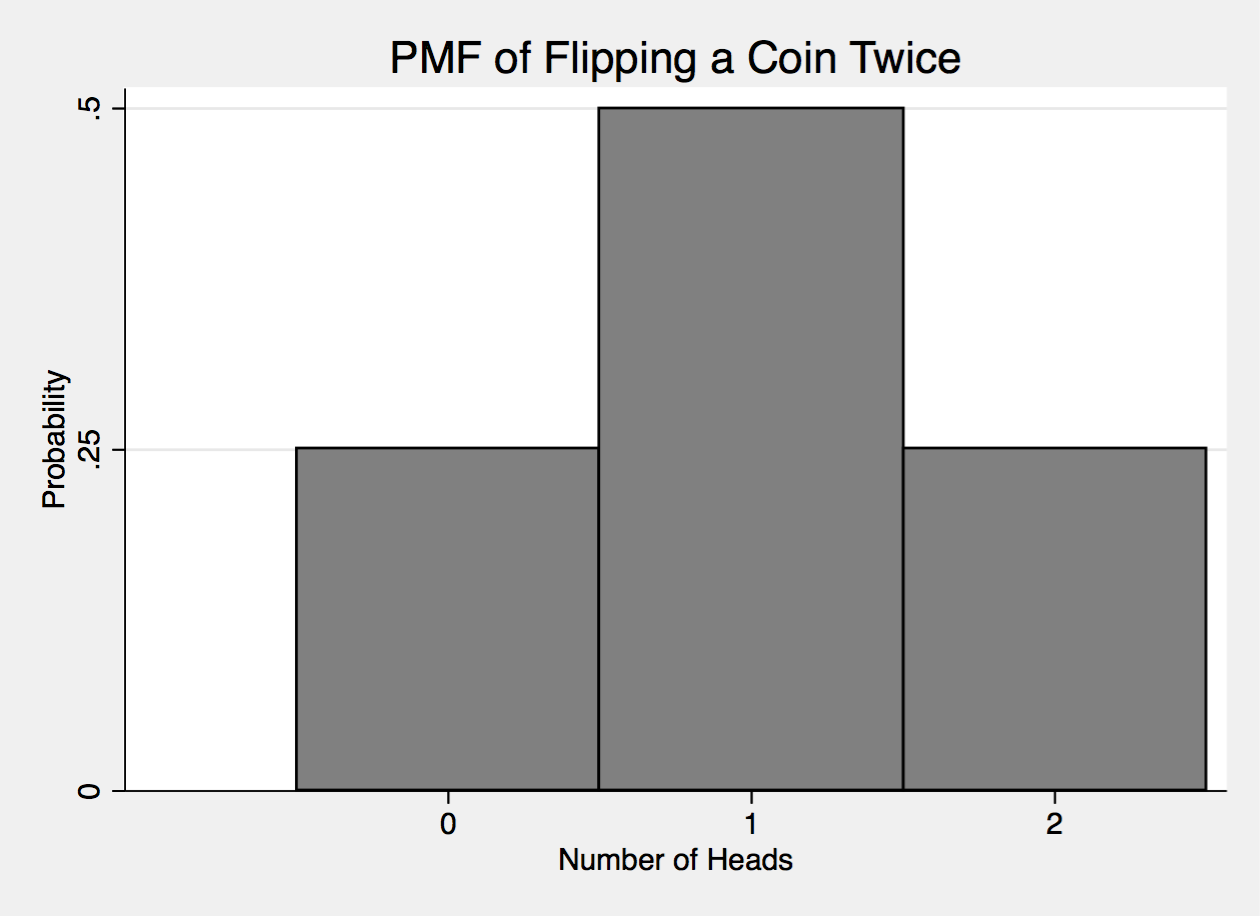
\includegraphics[width=.8\textwidth]{pmfcointwice.png}
\end{frame}

\begin{frame}{Properties of PMFs}
	We say a $p_X(x)$ is a \alert{valid} pmf if it satisfies the following:
				
	\begin{itemize}
		\item $0 \leq p_X(x) \leq 1$ for all $x \in S$.
		\item $\displaystyle\sum_{x \in S} p_X(x) = 1.$
	\end{itemize}
\end{frame}

\begin{frame}{Using PMFs}

	We can use the PMF to answer questions about cumulative probabilities, for example:
	Recall the previous example:

	\begin{center}
		\begin{tabular}{|c|c|}
			\hline
			X         & P(X) \\
			\hline
			1         & 0.07 \\
			2         & 0.36 \\
			3         & 0.32 \\
			4         & 0.21 \\
			5 or more & 0.04 \\
			\hline
		\end{tabular}
	\end{center}
	
	What is the probability a random table at the restaurant has 2 or 3 people seated?
	\[ 
		P(X=2) = 0.36 \text{ and } P(X=3) = 0.32 \implies 
	\]
	\[ 
		P(X=2 \text{ or } 3) = 0.36 + 0.32 = .68 
	\]
	
\end{frame}

\begin{frame}{Clicker Question}
	Assume there are four outcomes of $X$: $1, 5, 10$ and $20$. Given the following PMF, what is the probability X=20?
	\begin{center}
		\begin{tabular}{|c|c|}
			\hline
			X  & P(X) \\
			\hline
			1  & 0.42 \\
			5  & 0.23 \\
			10 & 0.18 \\
			20 & ??   \\
			\hline
		\end{tabular}
	\end{center}
	
	\begin{enumerate}[label=(\alph*)]
		\item 0.35
		\item 0.17
		\item 0.40
		\item Cannot be determined given the information
	\end{enumerate}
\end{frame}

\subsection{Continuous}
\begin{frame}{Defining Probability Density Function}
	Let $Y$ be a continuous random variable defined over the interval $[a,b]$.
		
	\begin{definition}[Probability Density Function]\vspace{2.5mm}
		The \alert{probability density function} (or pdf) of $Y$ is a function, $f_Y(y)$, that assigns a probability value to every possible \textit{interval} in $[a,b]$. We write
		\[ Pr(c\leqslant Y\leqslant d) = \int_{c}^{d}f_Y(y) dy, \]
		for all $(c,d)\subset [a,b]$.
	\end{definition}
\end{frame}
	

\begin{frame}{Example PDF}
	Suppose that $Y$ is a continuous random variable with pdf $f_Y(y) = 3y^2$ for $0<y<1$. What is $P(\frac{1}{4} \leqslant Y \leqslant \frac{1}{2})$?
				
	\centering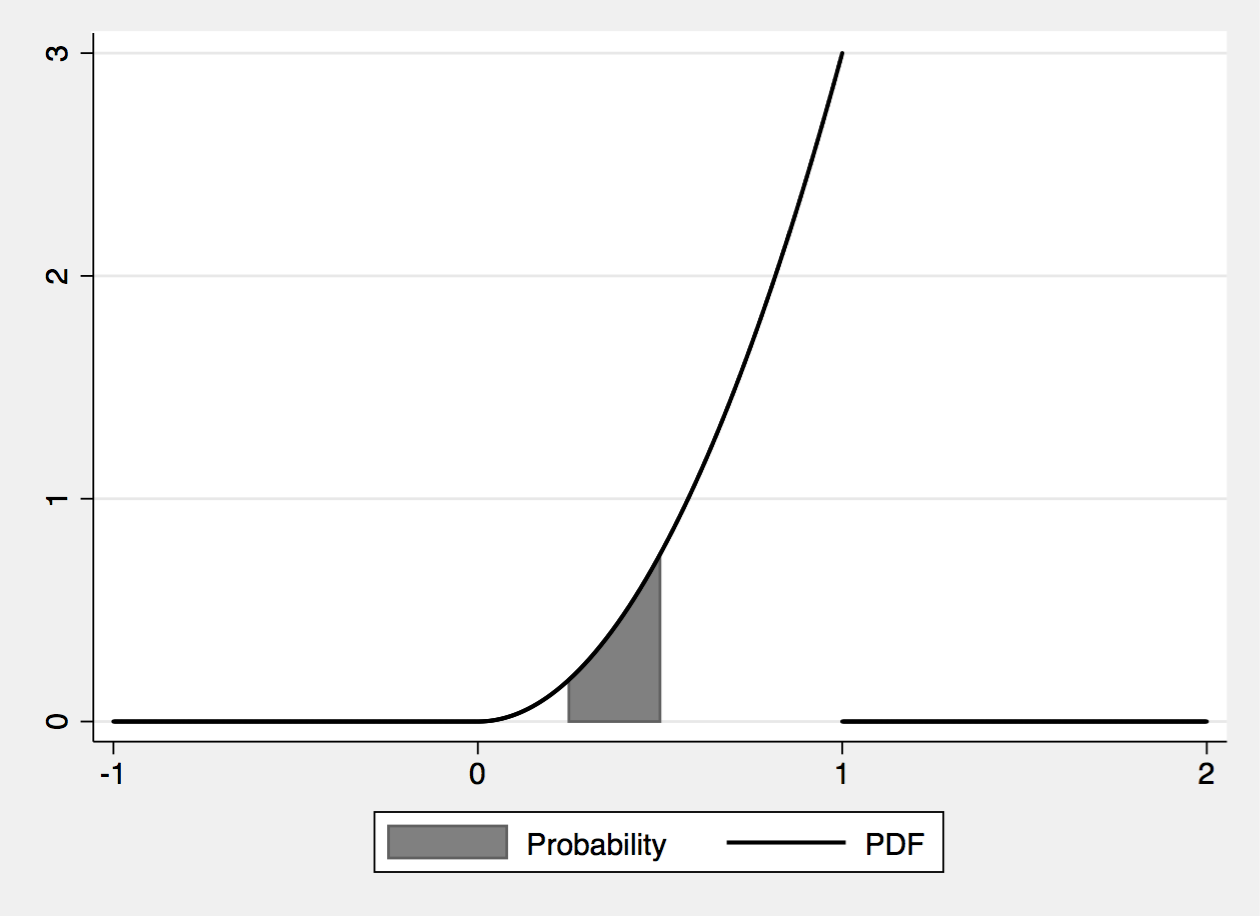
\includegraphics[width=.6\textwidth]{pdfwprob.png}
\end{frame}

\begin{frame}{Properties of PDFs}
	We say a $f_Y(y)$ is a \alert{valid} pdf if it satisfies the following:
			
	\begin{itemize}
		\item $0\leqslant \int f_Y(y) \leqslant 1$ for all $y \in [a,b]$.
		\item $\displaystyle\int_{a}^b f_Y(y)dy = 1.$
	\end{itemize}
			
	Note that by our construction, $Pr(Y=a) = \displaystyle\int_{a}^a f_Y(y)dy = 0$. 
		
	At first this might seem counterintuitive. But imagine trying to stop a stopwatch at exactly 30 seconds. What is the probability of that event?
\end{frame}

\begin{frame}{Clicker Question}
	Given the pdf, $f(y)=3y^2$ for $0<y<1$. What is the $P(Y<1/3)$?
		\begin{enumerate}[label=(\alph*)]
		\item $\frac{1}{3}$
		\item $\frac{1}{9}$
		\item $\frac{1}{27}$
		\item $\frac{26}{27}$
	\end{enumerate}
\end{frame}

\begin{frame}{Additional Example}
	Consider the probability distribution for random variable Y:
	\[ 
		f(y)= 8y, 0\leq y \leq \frac{1}{2} 
	\]

	\begin{enumerate}[label=(\alph*)]
		\item (4 points) Find $E[Y]$ \textit{$\rightarrow$ Expectation supplement}
		      
		\item (4 points) Find $P(Y<\frac{1}{3})$
		      		\item (4 points) Find $P(Y=\frac{1}{4})$
		      
		\item (4 points) Find $V[Y]$ \textit{$\rightarrow$ Expectation supplement}
		
		\item (4 points) Find $P(\frac{3}{4}<Y<1)$
	\end{enumerate}
\end{frame}


\end{document}